\chapter[Dynamic partitioning for SMR]{Dynamic partitioning for SMR}
\label{sec:dssmr}
% \section{Limitation of static partitioned SMR} \label{sec:ssmrproblem}


An inherent problem of traditional SMR is that it is not scalable: any replica
added to the system will deliver all requests, so throughput is not increased.
Scalable SMR addresses this issue in two ways: (i) by partitioning the
application state, while allowing every command to access (read/write) any
combination of partitions and (ii) using caching to reduce the communication
across partitions, while keeping the execution linearizable.

On the downside of this approach, as the number of multi-partition commands
increases, performance of \ssmr\ becomes worse, as partitions must communicate.
One way to reduce the number of multi-partition commands is by dynamically
changing the partitioning, putting variables that are usually accessed together
in the same partition. However, the partitioning oracle of \ssmr\ relies on a
static mapping of variables to partitions. One advantage of this implementation
is that all clients and servers can have their own local oracle, which always
returns a correct set of partitions for every query. Such a static mapping has
the major limitation of not allowing the service to dynamically adapt to
different access patterns. Any state reorganization requires system shutdown and
manual intervention.

Given these issues, it is crucial that highly available partitioned systems be
able to dynamically adapt to the workload. In this chapter, we present
\dssmrlong\ (\dssmr), a technique that allows a partitioned SMR system to
reconfigure its data placement on-the-fly. \dssmr\ achieves dynamic data
reconfiguration without sacrificing scalability or violating the properties of
classical SMR. These requirements introduce significant challenges. Since state
variables may change location, clients must find the current location of
variables. The scalability requirement rules out the use of a centralized oracle
that clients can consult to find out the partitions a command must be multicast
to. Even if clients can determine the current location of the variables needed
to execute a command, by the time the command is delivered at the involved
partitions one or more variables may have changed their location. Although the
client can retry the command with the new locations, how to guarantee that the
command will succeed in the second attempt? In classical SMR, every command
invoked by a non-faulty client always succeeds. \dssmr\ should provide similar
guarantees.

\dssmr\ was designed to exploit workload locality. Our scheme benefits from
simple manifestations of locality, such as commands that repeatedly access the
same state variables, and more complex manifestations, such as structural
locality in social network applications, where users with common interests have
a higher probability of being interconnected in the social graph. Focusing on
locality allows us to adopt a simple but effective approach to state
reconfiguration: whenever a command requires data from multiple partitions, the
variables involved are moved to a single partition and the command is executed
against this partition. To reduce the chances of skewed load among partitions,
the destination partition is chosen randomly. Although \dssmr\ could use more
sophisticated forms of partitioning, formulated as an optimization problem
(e.g., \cite{curino2010sch,taft2014est}), our technique has the advantage that
it does not need any prior information about the workload and is not
computationally expensive.

To track object locations without compromising scalability, in addition to a
centralized oracle that contains accurate information about the location of
state variables, each client caches previous consults to the oracle. As a
result, the oracle is only contacted the first time a client accesses a variable
or after a variable changes its partition. Under the assumption of locality, we
expect that most queries to the oracle will be accurately resolved by the
client's cache. To ensure that commands always succeed, despite concurrent
relocations, after attempting to execute a command a few times unsuccessfully,
\dssmr\ retries the command using \ssmr{}'s execution atomicity and involving
all partitions. Doing so increases the cost to execute the command but
guarantees that relocations will not interfere with the execution of the
command.

We have fully implemented \dssmr\ as the \dssmrlibname{} Java library, and we
performed a number of experiments using \dssmrappname{}, a social network
application built with \dssmrlibname{}. We compared the performance of \dssmr\
to \ssmr\ using different workloads. With a mixed workload that combines various
operations issued in a social network application, \dssmr\ reached 74~kcps
(thousands of commands per second), against less than 33~kcps achieved by
\ssmr{}, improving by a factor of over 2.2. Moreover, \dssmr's performance
scales with the number of partitions under all workloads.

The following contributions are presented in this chapter:
(1) It introduces \dssmr\ and discusses some performance optimizations, including
the caching technique.
(2) It details \dssmrlibname{}, a Java library to simplify the design of services based
on \dssmr{}.
(3) It describes \dssmrappname{} to demonstrate how \dssmrlibname{} can be used to implement
a scalable social network service.
(4) It presents a detailed experimental evaluation of \dssmrappname{}, deploying it with
\ssmr\ and \dssmr{} in order to compare the performance of the two replication
techniques.

The remainder of this chapter is organized as follows.
Section \ref{sec:dssmr-idea} gives an overview of \dssmr\.
Section \ref{sec:dssmr-detail} explains the algorithm in detail.
Section \ref{sec:dssmr-optm} proposes some performance optimizations.
Section \ref{sec:dssmr-correctness} argues about the correctness of the algorithm.
Section \ref{sec:dssmr-implementation} details the implementation of \dssmrlibname\.
Section \ref{sec:dssmr-experiments} reports on the performance of \dssmrlibname and \dssmrappname
Section \ref{sec:dssmr-conclusion} concludes the chapter.

\section{\dssmrlong}
\subsection{General idea}
\label{sec:dssmr-idea}

Dynamic \ssmr\ (\dssmr) defines a dynamic mapping of variables to partitions.
Each variable $v$ is mapped to partition $\ppm$, meaning that $v \in \ppm$. Such
a mapping is managed by a partitioning oracle, which is implemented as a
replicated service run by a group of server processes $\ssm_0$. The oracle
service allows the mapping of variables to partitions to be retrieved or changed
during execution. In more detail, \dssmr\ distinguishes five types of commands:
$access(\omega)$ is an application command that accesses (reads or writes)
variables in set $\omega \subseteq \vvm$ (as described in
Section~\ref{sec:sysmodel}), $create(v)$ creates a new variable $v$ and
initially maps it to a partition defined by the oracle, $delete(v)$ removes $v$
from the service state,
$move(v,\ppm_s,\ppm_d)$ moves variable $v$ from partition $\ppm_s$ to partition
$\ppm_d$, and $consult(C)$ asks the oracle which variables are accessed by
command $C$, and which partition contains each of them. The reply from the
oracle to a $consult$ command is called a $prophecy$. A prophecy usually
consists of a set of tuples $\langle v, \ppm \rangle$, meaning that variable $v$
is mapped to partition $\ppm$. The other possible values for a prophecy are $ok$
and $nok$, which mean that a command can and cannot be executed, respectively.

Clients can consult the oracle to know which partitions each command should be
multicast to, based on which variables are accessed by the command. If the reply
received from the oracle tells the client that the command accesses a single
partition, the client multicasts the command to that partition. If the command
accesses variables from multiple partitions, the client first multicasts one or
more $move$ commands to the oracle and to the involved partitions, with the
intent of having all variables in the same partition. Then, the command itself
is multicast to the one partition that now holds all variables accessed by the
command. If a subsequent command accesses the same variables, it will also
access a single partition. With this scheme, the access patterns of commands
will shape the mapping of variables to partitions, reducing the number of
multi-partition commands.

\begin{figure*}
\begin{minipage}[b]{1.0\linewidth}
\centering
      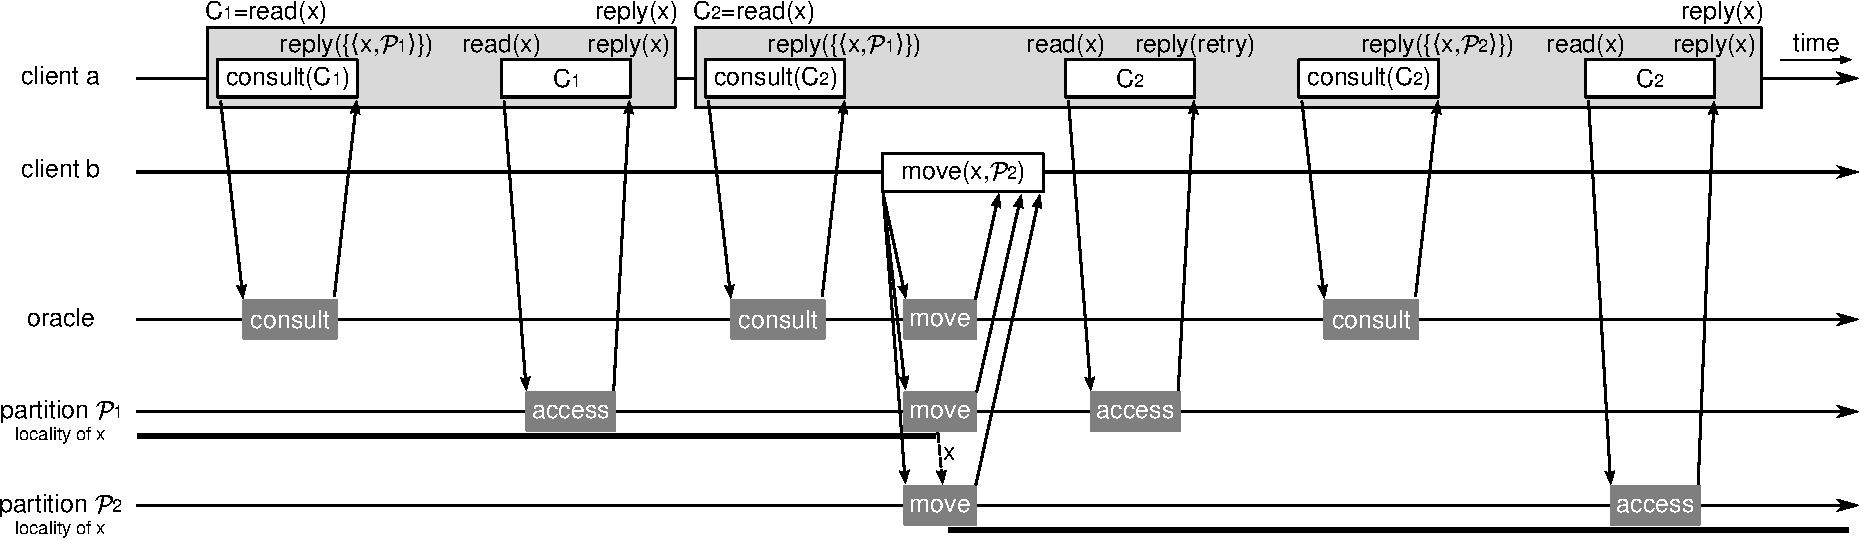
\includegraphics[width=0.8\linewidth]{figures/dssmr-detail}
\end{minipage}
\caption{Consulting the oracle and issuing a command are done in multiple calls to atomic-multicast.}
\label{fig:dssmr-detail}
\end{figure*}

Consulting the oracle and issuing the application command are done with separate
calls to atomic multicast in \dssmr{}. It may happen that, between those
operations, the partitioning changes. We illustrate this in
Figure~\ref{fig:dssmr-detail}. Commands $C_1$ and $C_2$ read variable $x$. Since
partitioning is dynamic, the client issuing the commands first consults the
oracle before multicasting each command. $C_1$ executes without the interference
of other commands, so consulting the oracle and multicasting the command only
once is enough for $C_1$ to be executed. However, before $C_2$ is multicast to
$\ppm_1$, another client issues a $move$ command that relocates $x$ to $\ppm_2$.
When $C_2$ is delivered at the servers of $\ppm_1$, the command is not executed,
since $x$ is not available at $\ppm_1$ anymore. A similar situation may arise
when a command accesses variables from multiple partitions, as it consists of
multicasting at least three commands separately: $consult$, $move$ and $access$.
The partitioning can change between the execution of any two of those commands.

To solve this problem, the client multicasts the set of variables accessed along
with each access command. Upon delivery, each server checks the set of variables
sent by the client. If all variables in the set belong to the local partition,
the command is executed; otherwise, a $retry$ message is sent back to the
client. When the client receives a $retry$ message, it consults the oracle
again, possibly moving variables across partitions, and then reissues the access
command. To guarantee termination, if the command fails a certain number of
times, the client multicasts the command to all partitions and the servers
execute it as in the original \ssmr{}.

The \dssmr\ client consists of the application logic and a client proxy.
The application does not see the state variables divided into partitions. When
the application issues a command, it sends the command to the proxy and
eventually receives a reply. All commands that deal with partitioning (i.e.,
consulting the oracle, moving objects across partitions and retrying commands as
described in the previous paragraph) are executed by the client proxy,
transparently to the application. When the client proxy multicasts a
partitioning-related command to multiple partitions and the oracle, partitions
and oracle exchange signals to ensure linearizability, as mentioned in
Section~\ref{sec:ssmr}. Every server and oracle process has its own \dssmr\
proxy as well. At each server, the proxy checks whether commands can be executed
and manages the exchange of data and signals between processes. At the oracle,
the service designer defines the application-dependent rules that must be
followed (e.g., where each variable is created at first) and a proxy is
responsible for managing the communication of the oracle with both clients and
servers when executing commands. \dssmr\ relies on a fault-tolerant multicast
layer for disseminating commands across replicas and implementing reliable
communication between partitions. Replies to commands are sent directly through
the network. Figure~\ref{fig:dssmr-arch} illustrates the architecture of \dssmr{}.

\begin{figure*}
\begin{minipage}[b]{1.0\linewidth}
\centering
      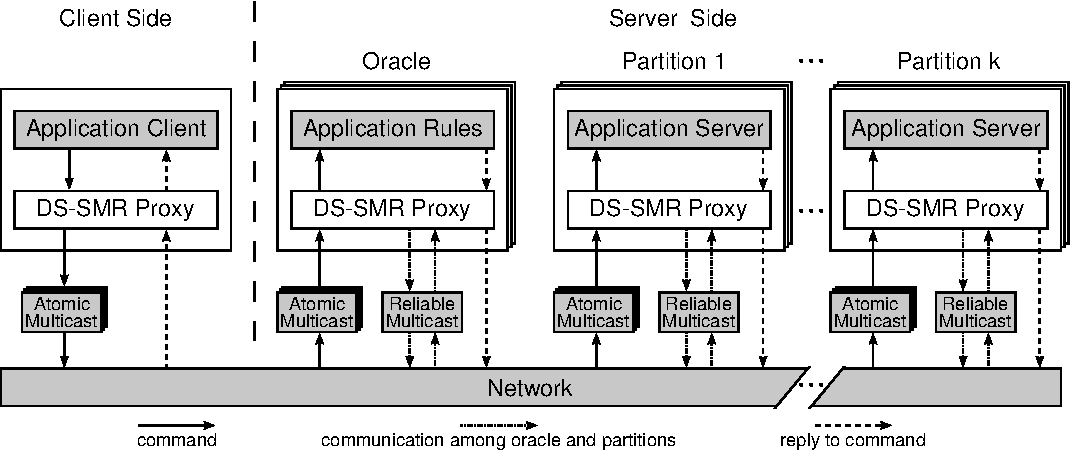
\includegraphics[width=0.8\linewidth]{figures/dssmr-arch}
\end{minipage}
\caption{The architecture of \dssmrlong{}.}
\label{fig:dssmr-arch}
\end{figure*}


\subsection{Detailed algorithm}
\label{sec:dssmr-detail}


When issuing a command, the application simply forwards the command to the
client proxy and waits for the reply. Consulting the oracle and multicasting the
command to different partitions is done internally by the proxy at the client.
Algorithms~\ref{alg:client_proxy}, \ref{alg:server_proxy}, and
\ref{alg:oracle_proxy} describe in detail how the \dssmr\ proxy works
respectively at client, server and oracle processes. Every server proxy at a
server in $\ssm_i$ has only partial knowledge of the partitioning: it knows only
which variables belong to $\ppm_i$. The oracle proxy has knowledge of every
$\ppm \in \Psi$. To maintain such a global knowledge, the oracle must \amdel{}
every command that creates, moves, or deletes variables. (In
Section~\ref{sec:dssmr-optm}, we introduce a caching mechanism to prevent the oracle
from becoming a performance bottleneck.)

\begin{algorithm}[t!]
\small

\begin{distribalgo}[1]

\vspace{1.0mm}

\INDENT{To issue a command $C$, the client proxy does:}

\vspace{1.0mm}

    \INDENT{\textbf{do}}
        \STATE \amcast$($oracle, $consult(C))$
        \STATE wait for $prophecy$
        \IF{$prophecy \in \{ok, nok\}$}
            \STATE $reply \leftarrow prophecy$
        \ELSE
            \STATE $C.dests \leftarrow \{\ppm : \exists \langle v, \ppm \rangle \in prophecy \}$
            \IF{$C$ is an $access(\omega)$ command and $|C.dests| > 1$}
                \STATE let $\ppm_d$ be one of the partitions in $C.dests$
                \label{algline:client:partition}
                \FOR{each $v \in \omega$}
                    \STATE // \textit{move $v$ to partition $\ppm_d$}
                    \STATE let $\ppm_s$ be $\ppm : \langle v, \ppm \rangle \in prophecy$
                    \IF{$\ppm_s \neq \ppm_d$}
                        \STATE $C_{move} \leftarrow move(v,\ppm_s,\ppm_d)$
                        \STATE $C_{move}.dests \leftarrow \{$oracle$,\ppm_s,\ppm_d\}$    
                        \STATE \amcast$(C_{move}.dests$, $C_{move})$
                    \ENDIF
                \ENDFOR
                \STATE $C.dests \leftarrow \{ \ppm_d \}$
            \ENDIF
            \IF{$C$ is $create$ or $delete$}
                \STATE $C.dests \leftarrow dests \cup \{oracle\}$
            \ENDIF
            \STATE \amcast$(C.dests$, $C)$
            \STATE wait for $reply$
        \ENDIF
    \ENDINDENT
    \STATE{\textbf{while} $reply = retry$ // \textit{after many retries, fall back to \ssmr}}
    \STATE return $reply$ to the application client
\ENDINDENT

\caption{\dssmr\ Client Proxy}
\label{alg:client_proxy}
\end{distribalgo}
\end{algorithm}

\textbf{The client proxy.} To execute a command $C$, the proxy first consults
the oracle. The oracle knows all state variables and which partition contains
each of them. Because of this, the oracle may already tell the client whether
the command can be executed or not. Such is the case of the $access(\omega)$
command: if there is a variable $v \in \omega$ that the command tries to read or
write and $v$ does not exist, the oracle already tells the client that the
command cannot be executed, by sending $nok$ as the prophecy. A $nok$ prophecy
is also returned for a $create(v)$ command when $v$ already exists. For a
$delete(v)$ command when $v$ already does not exist, an $ok$ prophecy is
returned. If the command can be executed, the client proxy receives a prophecy
containing a pair $\langle v, \ppm \rangle$, for every variable $v$ created,
accessed or deleted by the command. If the prophecy regarding an
$access(\omega)$ command contains multiple partitions, the client proxy chooses
one of them, $\ppm_d$, and tries to move all variables in $\omega$ to $\ppm_d$.
Then, the command $C$ itself is multicast to $\ppm_d$. As discussed in
Section~\ref{sec:dssmr-idea}, there is no guarantee that an interleave of
commands will not happen, even if the client waits for the replies to the move
commands. For this reason, and to save time, the client proxy multicasts all
move commands at once. Commands that change the partitioning (i.e., create and
delete) are also multicast to the oracle. If the reply received to the command
is $retry$, the procedure restarts: the proxy consults the oracle again,
possibly moves variables across partitions, and multicasts $C$ to the
appropriate partitions once more. After reaching a given threshold of retries
for $C$, the proxy falls back to \ssmr{}, multicasting $C$ to all partitions
(and the oracle, in case $C$ is a create or delete command), which ensures the
command's termination.

\begin{algorithm}[t!]
\small

\begin{distribalgo}[1]

\vspace{1.0mm}

\INDENT{To execute a command $C$, the server proxy in partition $\ppm$ does:}

    \vspace{1.0mm}
    
    \INDENT{\textbf{when} \rmdel$( \langle val, C \rangle )$}
        \STATE $rcvd\_msgs \leftarrow rcvd\_msgs \cup \{\langle val, C \rangle\}$
    \ENDINDENT

    \vspace{1.0mm}

    \INDENT{\textbf{when} \amdel$(C)$}

    \vspace{1.0mm}

        \IF{\underline{$C$ is an $access(\omega)$ command}}
            \IF{$\exists v \in \omega : v \not\in \ppm$}
                \STATE reply with $retry$
            \ELSE
                \STATE have the command executed by the application server
                \STATE send the reply to the client
            \ENDIF
        

        \vspace{1.0mm}
    
        \ELSIF{\underline{$C$ is a $move(v,\ppm_s,\ppm_d)$ command}}
            \IF{$\ppm = \ppm_s$}
                \IF{$v \in \ppm$}
                    \STATE \rmcast$(\ppm_d$,$\langle v, C \rangle)$
                    \STATE $\ppm \leftarrow \ppm \setminus \{v\}$
                \ELSE
                    \STATE \rmcast$(\ppm_d$,$\langle null, C \rangle)$
                \ENDIF
            \ELSE
                \STATE wait until $\exists val : \langle val, C \rangle \in rcvd\_msgs$
                \IF{$val \neq null$}
                    \STATE $v \leftarrow val$
                    \STATE $\ppm \leftarrow \ppm \cup \{v\}$
                \ENDIF
            \ENDIF
        
        \vspace{1.0mm}
    
        \ELSIF{\underline{$C$ is a $create(v)$ command}}
            \STATE wait until $\langle val, C \rangle \in rcvd\_msgs$
            \IF{$val = ok$}
                \STATE $\ppm \leftarrow \ppm \cup \{v\}$
%                \STATE reply with $success$
%            \ELSE
%                \STATE reply with $retry$
            \ENDIF
        
        \vspace{1.0mm}
        
        \ELSIF{\underline{$C$ is a $delete(v)$ command}}
            \IF{$v \in \ppm$}
                \STATE $\ppm \leftarrow \ppm \setminus \{v\}$
%                \STATE reply with $success$
%            \ELSE
%                \STATE reply with $retry$
            \ENDIF
        \ENDIF
    \ENDINDENT
\ENDINDENT

\caption{\dssmr\ Server Proxy}
\label{alg:server_proxy}
\end{distribalgo}
\end{algorithm}

\textbf{The server proxy.} Upon delivery, access commands are intercepted by the
\dssmr\ proxy before they are executed by the application server. In \dssmr{},
every access command is executed in a single partition. If a server proxy in
partition $\ppm$ intercepts an $access(\omega)$ command that accesses a variable
$v \in \omega$ that does not belong to $\ppm$, it means that the variable is in
some other partition, or it does not exist. Either way, the client should retry
with a different set of partitions, if the variable does exist. To execute a
$delete(v)$ command, the server proxy at partition $\ppm$ simply removes $v$
from partition $\ppm$, in case $v \in \ppm$. In case $v \not\in \ppm$, it might
be that the variable exists but belongs to some other partition $\ppm'$. Since
only the oracle and the servers at $\ppm'$ have this knowledge, it is the oracle
who replies to delete commands.

\dssmr\ server and oracle proxies coordinate to execute commands that create or
move variables. Such coordination is done by means of \rmcast{}. When a
$create(v)$ command is delivered at $\ppm$, the server proxy waits for a message
from the oracle, telling whether the variable can be created or not, to be
\rmdel{}ed. Such a message from the oracle is necessary because $v$ might not
belong to $\ppm$, but it might belong to some other partition $\ppm'$ that
servers of $\ppm$ have no knowledge of. If the create command can be executed,
the oracle can already reply to the client with a positive acknowledgement,
saving time. This can be done because atomic multicast guarantees that all
non-faulty servers at $\ppm$ will eventually deliver and execute the command. As
for move commands, each $move(v,\ppm_s,\ppm_d)$ command consists of moving
variable $v$ from a source partition $\ppm_s$ to a destination partition
$\ppm_d$. If the server's partition $\ppm$ is the source partition (i.e., $\ppm$
= $\ppm_s$), the server proxy checks whether $v$ belongs to $\ppm$. If $v \in
\ppm$, the proxy \rmcast{}s $\langle v, C \rangle$ to $\ppm_d$, so that servers
at the destination partition know the most recent value of $v$; $C$ is sent
along with $v$ to inform which move command that message is related to. If $v
\not\in \ppm$, a $\langle null, C \rangle$ message is \rmcast\ to $\ppm_d$,
informing $\ppm_d$ that the move command cannot be executed.

\begin{algorithm}[t!]
\small

\begin{distribalgo}[1]

\vspace{1.5mm}

\INDENT{To execute a command $C$, the oracle proxy does:}

    \vspace{1.5mm}

    \INDENT{\textbf{when} \amdel$(C)$}

    \vspace{1.5mm}

        \IF{\underline{$C$ is a $consult(C_c)$ command}}
            \STATE $prophecy \leftarrow \emptyset$

            \IF{$C_c$ is an $access(\omega)$ command}
                \IF{$\exists v \in \omega : (\nexists \ppm \in \Psi : v \in \ppm)$}
                    \STATE $prophecy \leftarrow nok$
                \ELSE
                    \FOR{each $v \in \omega$}
                        \STATE $prophecy \leftarrow prophecy \cup \{\langle v, \ppm \rangle \}:v \in \ppm$
                    \ENDFOR
                \ENDIF

            \ELSIF{$C_c$ is a $create(v)$ command}
                \IF{$\exists \ppm \in \Psi : v \in \ppm$}
                    \STATE $prophecy \leftarrow nok$
                \ELSE
                    \STATE $\ppm \leftarrow$ initial partition, defined by application rules
                    \STATE $prophecy \leftarrow \{\langle v, \ppm \rangle \}$
                \ENDIF

            \ELSIF{$C_c$ is a $delete(v)$ command}
                \IF{$\nexists \ppm \in \Psi : v \in \ppm$}
                    \STATE $prophecy \leftarrow ok$
                \ELSE
                    \STATE $prophecy \leftarrow \{\langle v, \ppm \rangle \} : v \in \ppm$
                \ENDIF
                
            \ENDIF
            
            \STATE send $prophecy$ to the client

        \vspace{1.5mm}

        \ELSIF{\underline{$C$ is a $move(v,\ppm_s,\ppm_d)$ command}}
            \IF{$v \in \ppm_s$}
                \STATE $\ppm_s \leftarrow \ppm_s \setminus \{v\}$
                \STATE $\ppm_d \leftarrow \ppm_d \cup      \{v\}$
            \ENDIF

        \vspace{1.0mm}
    
        \ELSIF{\underline{$C$ is a $create(v)$ command}}
            \STATE let $\ppm_c$ be $\ppm : \{\ppm\} = C.dests \setminus \{$oracle$\}$
            \IF{$\nexists \ppm \in \Psi : v \in \ppm$}
                \STATE $outcome \leftarrow ok$
            \ELSE
                \STATE $outcome \leftarrow nok$
            \ENDIF
            \STATE \rmcast$(\ppm_c, \langle outcome, C \rangle )$
            \STATE send $outcome$ to the client
        
        \vspace{1.0mm}
        
        \ELSIF{\underline{$C$ is a $delete(v)$ command}}
            \STATE let $\ppm_d$ be $\ppm : \{\ppm\} = C.dests \setminus \{$oracle$\}$
            \IF{$\nexists \ppm \in \Psi: v \in \ppm$ or $v \in \ppm_d$}
                \STATE send $ok$    to the client
            \ELSE
                \STATE send $retry$ to the client
            \ENDIF
            
            
        \ENDIF
    \ENDINDENT
\ENDINDENT

\caption{\dssmr\ Oracle Proxy}
\label{alg:oracle_proxy}
\end{distribalgo}
\end{algorithm}

\textbf{The oracle proxy.} One of the purposes of the oracle proxy is to make
prophecies regarding the location of state variables. Such prophecies are used
by client proxies to multicast commands to the right partitions. A prophecy
regarding an $access(\omega)$ command contains, for each $v \in \omega$, a pair
$\langle v, \ppm \rangle$, meaning that $v \in \ppm$. If any of the variables in
$\omega$ does not exist, the prophecy already tells the client that the command
cannot be executed (with a $nok$ value). For a $create(v)$ command, the prophecy
tells where $v$ should be created, based on rules defined by the application, if
$v$ does not exist. If $v$ already exists, the prophecy will contain $nok$, so
that the client knows that the create command cannot be executed. The prophecy
regarding a $delete(v)$ command contains the partition that contains $v$, or
$ok$, in case $v$ was already deleted or never~existed.

Besides dispensing prophecies, the oracle is responsible for executing create,
move, and delete commands, coordinating with server proxies when necessary, and
replying directly to clients in some cases. For each $move(v,\ppm_s,\ppm_d)$
command, the oracle checks whether $v$ in fact belongs to the source partition
$\ppm_s$. If that is the case, the command is executed, moving $v$ to $\ppm_d$.
Each $create(v)$ command is multicast to the oracle and to a partition $\ppm$.
If $v$ already exists, the oracle tells $\ppm$ that the command cannot be
executed, by \rmcast{}ing $nok$ to $\ppm$. The oracle also sends $nok$ to the
client as reply, meaning that $v$ already exists. If $v$ does not exist, the
oracle tells $\ppm$ that the command can be executed, by \rmcast{}ing $ok$ to
$\ppm$. It also tells the client that the command succeeded with an $ok$ reply.
Finally, each $delete(v)$ command is multicast to the oracle and to a partition
$\ppm$, where the client proxy assumed $v$ to be located. If $v$ belongs to
$\ppm$, or $v$ does not exist, the oracle tells the client that the delete
command succeeded. Otherwise, that is, if $v$ exists, but $delete(v)$ was
multicast to the wrong partition, the oracle tells the client to retry.



\subsection{Performance optimizations}
\label{sec:dssmr-optm}

In this section, we introduce two optimizations for \dssmr{}: caching and load
balancing.

\textbf{Caching.} In Algorithm~\ref{alg:client_proxy}, for every command issued
by the client, the proxy consults the oracle. If every command passes by the
oracle, the system is unlikely to scale, as the oracle is prone to becoming a
bottleneck. To provide a scalable solution, each client proxy has a local cache
of the partitioning information. Before multicasting an application command $C$
to be executed, the client proxy checks whether the cache has information about
every variable concerned by $C$. If the cache does have such a knowledge, the
oracle is not consulted and the information contained in the cache is used
instead. If the reply to $C$ is $retry$, the oracle is consulted and the
returned prophecy is used to update the client proxy's cache.
Algorithm~\ref{alg:client_proxy} is followed from the second attempt to execute
$C$ on. The cache is a local service that follows an algorithm similar to that
of the oracle, except it responds only to $consult(C)$ commands and, in
situations where the oracle would return $ok$ or $nok$, the cache tells the
client proxy to consult the actual oracle.


Naturally, the cached partitioning information held by the client proxy may be
outdated. On the one hand, this may lead a command to be multicast to the
wrong set of partitions, which will incur in the client proxy having to
retry executing the command. For instance, in Figure~\ref{fig:dssmr-retry} the
client has an outdated cache, incurring in a new consultation to the oracle
when executing $C_3$. On the other hand, the client proxy may already have to
retry commands, even if the oracle is always consulted first, as shown in
Figure~\ref{fig:dssmr-detail}. If most commands are executed without consulting
the oracle, as in the case of $C_4$ in Figure~\ref{fig:dssmr-retry}, we avoid
turning the oracle into a bottleneck. Moreover, such a cache can be updated
ahead of time, not having to wait for an actual application command to be issued
to only then consult the oracle. This way, the client proxy can keep a cache of
partitioning information of variables that the proxy deems likely to be accessed
in the future.

\textbf{Load balancing}. When moving variables, the client proxies may try to
distribute them in a way that balances the workload among partitions. This way,
the system is more likely to scale throughput with the number of server groups.
One way of balancing load is by having roughly the same number of state
variables in every partition. This can be implemented by having client proxies
choosing randomly the partition that will receive all variables concerned by
each command (at line~\ref                {algline:client:partition} of
Algorithm~\ref{alg:client_proxy}). Besides improving performance, balancing the
load among partitions prevents the system from degenerating into a
single-partition system, with all variables being moved to the same place as
commands are executed.


\begin{figure*}
\begin{minipage}[b]{1\linewidth} % A minipage that covers the whole width of the
page
\centering
      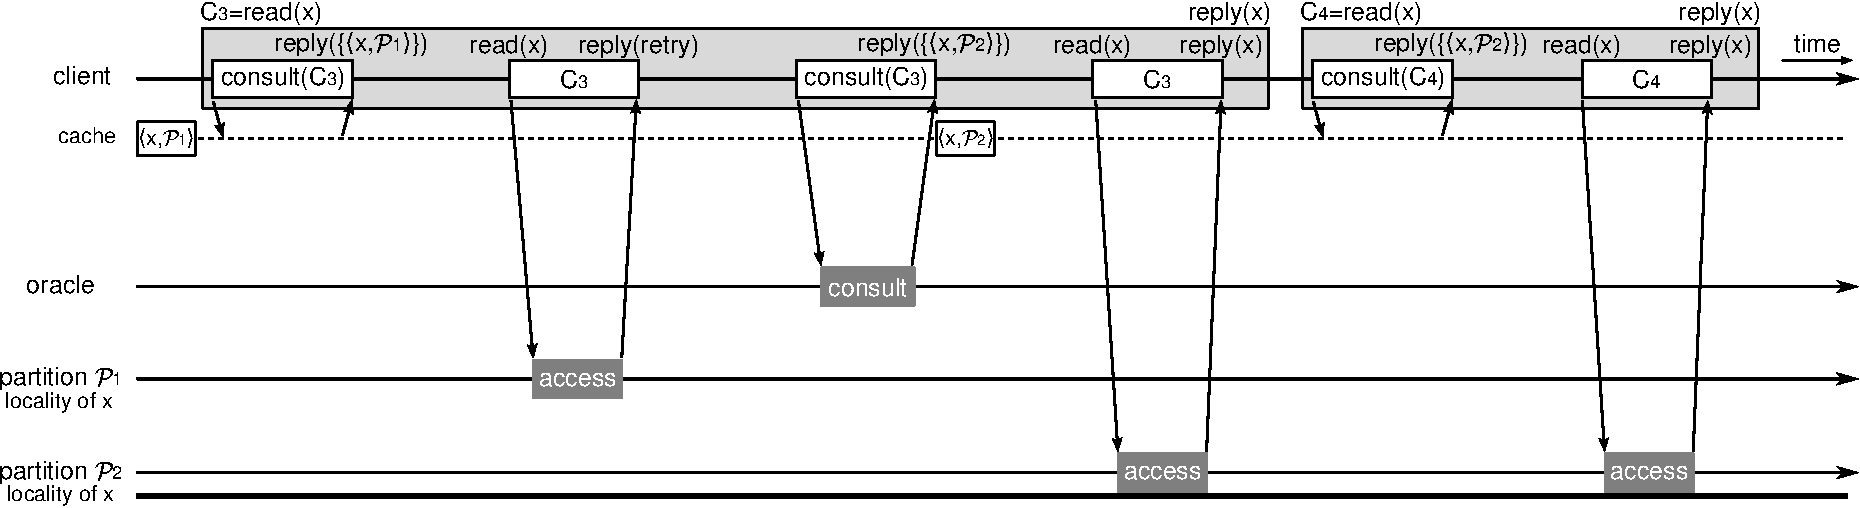
\includegraphics[width=1.0\linewidth]{figures/dssmr-retry}
\end{minipage}
\caption{Each client proxy in \dssmr\ maintains a cache in order to avoid  consulting the oracle. White boxes represent actions of the client proxy.}
\label{fig:dssmr-retry}
\end{figure*}


\subsection{Correctness}
\label{sec:dssmr-correctness}

In this section, we argue that \dssmr\ ensures termination and linearizability.
By ensuring termination, we mean that for every command $C$ issued by a correct
client, a reply to $C$ different than $retry$ is eventually received by the
client. This assumes that at least one oracle process is correct and that every
partition has at least one correct server. Given these constraints, the only
thing that could prevent a command from terminating would be an execution that
forced the client proxy to keep retrying a command. This problem is trivially
solved by falling back to \ssmr\ after a predefined number of retries: at a
certain point, the client proxy multicast the command to all server and oracle
processes, which execute the command as in \ssmr{}, i.e., with coordination
among all partitions and the oracle.

As for linearizability, we argue that, if every command in execution \ex\ of
\dssmr\ is delivered by atomic multicast and is \emph{execution atomic} (as
defined in~\cite{bezerra2014ssmr}), then \ex\ is linearizable. We denote the
order given by atomic multicast by relation $\prec$. Given any two messages
$m_1$ and $m_2$, ``$m_1 \prec m_2$'' means that there exists a process that
delivers both messages and $m_1$ is delivered before $m_2$, or there is some
message $m'$ such that $m_1 \prec m'$ and $m' \prec m_2$, which can be written
as \mbox{$m_1 \prec m' \prec m_2$}.
%\fxnote[draft]{use the phrase \"there exists a process that\" }
Also, for the purposes of this proof, we consider the oracle to be a partition,
as it also \amdel{}s and executes application commands.

Suppose, by means of contradiction, that there exist two commands $x$ and $y$,
where $x$ finishes before $y$ starts, but $y \prec x$ in the execution. There
are two possibilities to be considered: (i) $x$ and $y$ are delivered by the
same process $p$, or (ii) no process delivers both $x$ and $y$.

In case (i), at least one process $p$ delivers both $x$ and $y$. As $x$ finishes
before $y$ starts, then $p$ delivers $x$, then $y$. From the properties of
atomic multicast, and since each partition is mapped to a multicast group, no
process delivers $y$, then $x$. Therefore, we reach a contradiction in this
case.

In case (ii), if there were no other commands in \ex, then the execution of $x$
and $y$ could be done in any order, which would contradict the supposition that
$y \prec x$. Therefore, there are commands $z_1, ..., z_n$ with atomic order $y
\prec z_1 \prec \cdots \prec z_n \prec x$, where some process $p_0$ (of
partition $\ppm_0$) delivers $y$, then $z_1$; some process $p_1 \in \ppm_1$
delivers $z_1$, then $z_2$, and so on: process $p_i \in \ppm_i$ delivers
$z_{i}$, then $z_{i+1}$, where $1 \leq i < n$. Finally, process $p_n \in \ppm_n$
delivers $z_n$, then $x$.

Let $z_0 = y$ and let $atomic(i)$ be the following predicate: ``For every
process $p_i \in \ppm_i$, $p_i$ finishes executing $z_i$ only after some $p_0
\in \ppm_0$ started executing $z_0$.'' We now claim that $atomic(i)$ is true for
every $i$, where $0 \leq i \leq n$. We prove our claim by induction.

%\begin{itemize}

%\item
\emph{Basis ($i=0$)}: $atomic(0)$ is obviously true, as $p_0$ can only finish
executing $z_0$ after starting executing it.

%\item
\emph{Induction step}: If $atomic(i)$, then $atomic(i+1)$. \\
Proof: Command $z_{i+1}$ is multicast to both $\ppm_i$ and $\ppm_{i+1}$. Since
$z_{i+1}$ is execution atomic, before any $p_{i+1} \in \ppm_{i+1}$ finishes
executing $z_{i+1}$, some $p_i \in \ppm_i$ starts executing $z_{i+1}$. Since
$z_i \prec z_{i+1}$, every $p_i \in \ppm_i$ start executing $z_{i+1}$ only after
finishing the execution of $z_i$. As $atomic(i)$ is true, this will only happen
after some $p_0 \in \ppm_0$ started executing $z_0$.

%\end{itemize}

As $z_n \prec x$, for every $p_n \in \ppm_n$, $p_n$ executes command $x$ only
after the execution of $z_n$ at $p_n$ finishes. From the above claim, this
happens only after some $p_0 \in \ppm_0$ starts executing $y$. This means that
$y$ ($z_0$) was issued by a client before any client received a response for
$x$, which contradicts the assumption that $x$ precedes $y$ in real-time, i.e.,
that command $y$ was issued after the reply for command $x$ was received.


\section{Implementation}
\label{sec:dssmr-implementation}

In this section, we describe \dssmrlibname{}, a library that implements both \ssmr\
and \dssmr{}, and \dssmrappname{}, a scalable social network application built with
\dssmrlibname{}. \dssmrlibname\ and \dssmrappname\ were both implemented in Java.

\subsection{\dssmrlibname}

To implement a replicated service with \dssmrlibname{}, the developer (i.e., service
designer) must extend three classes: PRObject, StateMachine, OracleStateMachine.

\textbf{The PRObject class.} \dssmrlibname{} supports partial replication (i.e., some
objects may be replicated in some partitions, not all). Therefore, when
executing a command, a replica might not have local access to some of the
objects involved in the execution of the command. The developer informs
\dssmrlibname{} which object classes are partially replicated by extending the
PRObject class. Each object of such a class is stored either locally or remotely,
but the application code is agnostic to that. All calls to methods of such
objects are intercepted by \dssmrlibname{}, transparently to the developer.

% are you still using the aspect? do methods actually get intercepted by
% D-Eyrie?

\textbf{The StateMachine class.} This class implements the logic of the server
proxy. The application server class must extend the StateMachine class. To
execute commands, the developer must provide an implementation for the method
executeCommand(Command). The code for such a method is agnostic to the existence
of partitions. In other words, it can be exactly the same as the code used to
execute commands with classical state machine replication (i.e., full
replication). \dssmrlibname{} is responsible for handling all communication between
partitions and oracle transparently. To start the server, method
runStateMachine() is called. Method createObject() also needs to be implemented,
where the developer defines how new state objects are loaded or created.

\textbf{The OracleStateMachine class.} This class implements the logic of the
oracle proxy. It extends StateMachine, so the oracle can be deployed similarly
to a fault-tolerant partition in the original \ssmr{}. Class OracleStateMachine
has a default implementation, but the developer is encouraged to override its
methods. Method extractObject(Command) returns the set of objects accessed by
the command. It should be overridden by the application so that the client proxy
can relocate all necessary objects to a destination partition before executing
the application command.
% didn't understand this: ``in the case there are hidden objects in the command.''
Method getTargetPartition(Set$\langle$Object$\rangle$) returns a particular
partition to which objects should be moved, when they are not in the same
partition yet, in order to execute an application command that accesses those
objects. The default implementation of the method returns a random partition.
The developer can override it in order to further improve the distribution of
objects among partitions. For instance, the destination partition could be
chosen based on an attribute of the objects passed to the method.

The client proxy is implemented in class Client, which handles all communication
of the application client with the partitioned service. The client proxy
provides methods \emph{sendCreate(Command, Callback)}, \emph{sendAccess(Command,
Callback)}, and \emph{sendDelete(Command, Callback)}. The client proxy's default
behavior is to keep retrying commands (and fallback to \ssmr\ in case of too
many retries) and only call back the application client when the command has
been successfully executed. However, the developer can change this behavior by
overriding the error() method of Callback. The error() method is called when a
$retry$ reply is received.

% i don't understand what the application can actually change with the error()
% method

\subsection{\dssmrappname}

We implemented \dssmrappname{}, a social network application similar to Twitter,
using \dssmrlibname{}. Twitter is an online social networking service in which users
can post 140-character messages and read posted messages of other users. The API
consists basically of: post (user publishes a message), follow (user starts
following another user), unfollow (user stops following someone), and
getTimeline (user requests messages of all people whom the user follows).

State partitioning in \dssmrappname\ is based on users' interest. A function $f(uid)$
returns the partition that user with id $uid$ should belong to, based on the
user's interest. Function $f$ is implemented in method getObjectPlacement(User)
of class \dssmrappname{}Oracle, which extends OracleStateMachine (class User extends
PRObject). Taking into account that a typical user probably spends more time
reading messages (i.e., issuing getTimeline) than writing them (i.e., issuing
post), we decided to optimize getTimeline to be single-partition. This means
that, when a user requests his or her timeline, all messages should be available
in the partition that stores that user's data, in the form of a materialized
timeline (similarly to a materialized view in a database). To make this
possible, whenever a post request is executed, the message is inserted into the
materialized timeline of all users that follow the one that is posting. Also,
when a user starts following another user, the messages of the followed user are
inserted into the follower's materialized timeline as part of the command
execution; likewise, they are removed when a user stops following another user.
Because of this design decision, every getTimeline request accesses only one
partition, follow and unfollow requests access objects on at most two
partitions, and post requests access up to all partitions. The \dssmrappname{} client
does not need any knowledge about partitions, since it uses method
sendAccessCommand(command) of the \dssmr{} client proxy to issue its commands.

One detail about the post request is that it needs access to all users that
follow the user issuing the post.
%Thus the list of follower need to be attached in the post command. However, the
%(Chirper) client cannot know for sure who follows the user: it keeps a cache of
%followers, but such cache can become stale if a different user starts following
%the poster.
To ensure linearizability when executing a post request, the \dssmrappname\ server
overrides the extractObject(command) method to check if all followers that will
be accessed by the command are available in the local partition (i.e., the
partition of the server executing the post command). If this is the case, the
request is executed. Otherwise, the server sends a $retry(\gamma)$ message,
where $\gamma$ is the complete set of followers of the user who was posting.
Then, the \dssmrappname\ server proceeds to the next command. Upon receiving the
$retry(\gamma)$ message, the client proxy tries to move all users in $\gamma$ to
the same partition before retrying to execute the post command.


\section{Performance evaluation}
\label{sec:dssmr-experiments}

In this section, we present the results found for \dssmrappname\ with different
loads and partitionings and compare them with the original
\ssmr{}~\cite{bezerra2014ssmr}. In these experiments, we are interested in
assessing \dssmr{}'s performance with workloads that present different levels of
locality. By locality, we mean the likelihood that certain groups of data items
are accessed together (by the same command). In
Section~\ref{sec:dssmr-evaluation:setup}, we describe the environment where we
conducted our experiments. In Section~\ref{sec:dssmr-evaluation:strongloc}, we
show the results with strong-locality workloads.
In Section~\ref{sec:dssmr-evaluation:weakloc}, we show the results for
weak-locality workloads.

\begin{figure*}
\begin{minipage}[b]{1\linewidth}
\centering
      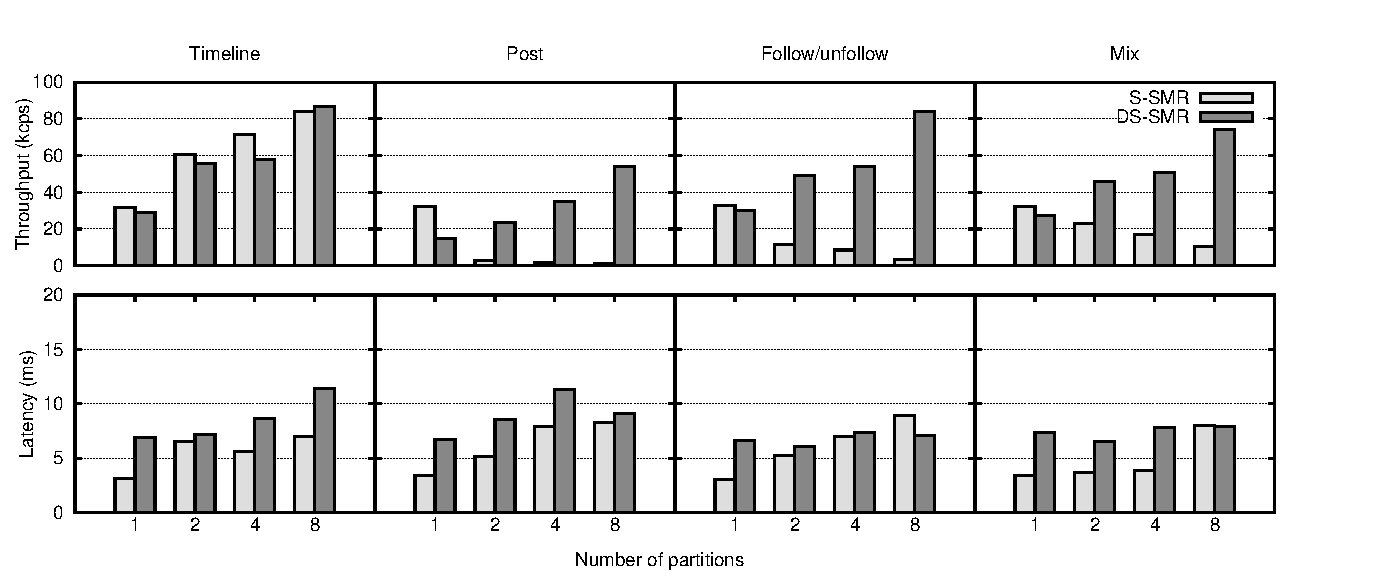
\includegraphics[width=1\linewidth]{figures/experiments/dssmr/strong-locality}
\end{minipage}
\caption{Results of \dssmrappname\ running with \ssmr\ and \dssmr{} with strong-locality workload. Throughput is shown in thousands of commands per second (kcps).}
\label{fig:dssmr-strongloc}
\end{figure*}


\begin{figure*}
\begin{minipage}[b]{1\linewidth}
\centering
      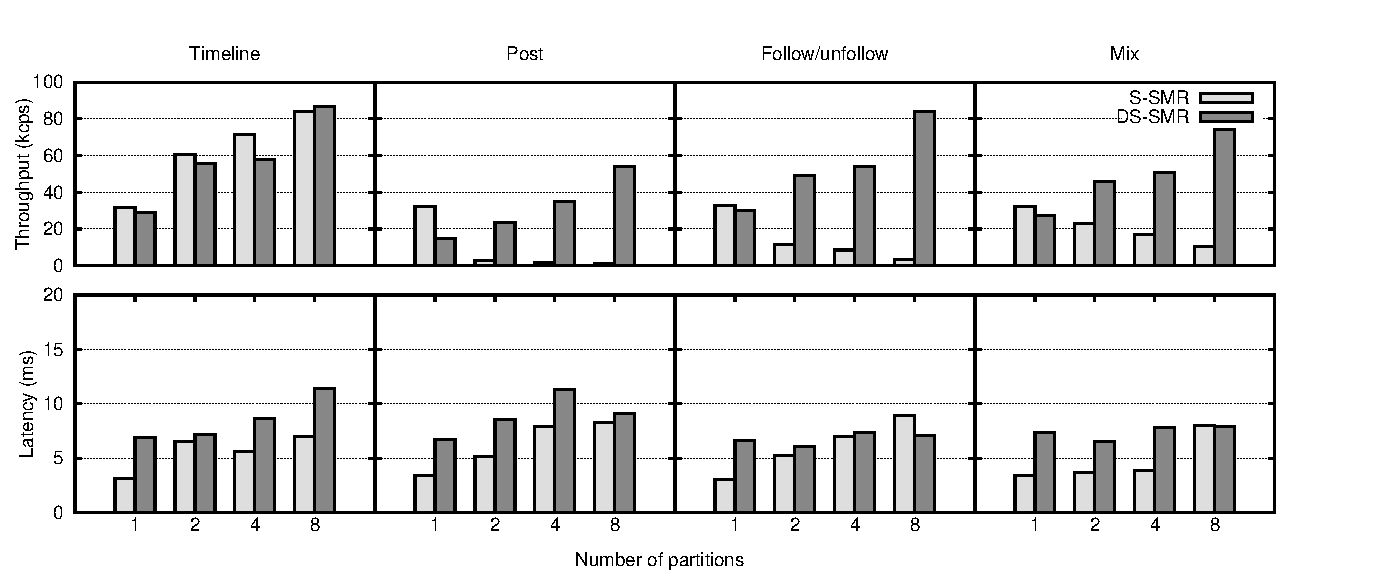
\includegraphics[width=1\linewidth]{figures/experiments/dssmr/weak-locality}
\end{minipage}
\caption{Results of \dssmrappname\ running with \ssmr\ and \dssmr{} with weak-locality workload. Throughput is shown in thousands of commands per second (kcps).}
\label{fig:dssmr-weakloc}
\end{figure*}

\subsection{Environment setup and configuration parameters}
\label{sec:dssmr-evaluation:setup}

We conducted all experiments on a cluster that had two types of nodes: (a) HP
SE1102 nodes, equipped with two Intel Xeon L5420 processors running at 2.5 GHz
and with 8 GB of main memory, and (b) Dell SC1435 nodes, equipped with two AMD
Opteron 2212 processors running at 2.0 GHz and with 4 GB of main memory. The HP
nodes were connected to an HP ProCurve 2920-48G gigabit network switch, and the
Dell nodes were connected to another, identical switch. Those switches were
interconnected by a 20 Gbps link. All nodes ran CentOS Linux 7.1 with kernel
3.10 and had the OpenJDK Runtime Environment~8 with the \mbox{64-Bit} Server VM
(build 25.45-b02).
%We kept the clocks synchronized using NTP in order to measure latency
%components involving events in different computers.

For the experiments, we use the following workloads: Timeline (composed only of
getTimeline requests), Post (only post requests), Follow/unfollow (50\% of
follow requests and 50\% of unfollow), and Mix (7.5\% post, 3.75\% follow,
3.75\% unfollow, and 85\% getTimeline).

\subsection{Results for strong locality}
\label{sec:dssmr-evaluation:strongloc}

% THROUGHPUT

We can see in Figure~\ref{fig:dssmr-strongloc} and Table~\ref{tbl:results} the
results achieved with \dssmrappname{}, running with a strong-locality workload.
For the Timeline workload, the throughput with \dssmr\ and \ssmr\ are very
similar. This happens because getTimeline requests are optimized to be
single-partition: all posts in a user's timeline are stored along with the User
object. Every getTimeline requests accesses a single User object (of the user
whose timeline is being requested). This is the ideal workload for \ssmr{}. In
\dssmr{}, the partitioning does not change, and consulting the oracle becomes
unnecessary thanks to the local cache at each client. This happens because there
are no other commands in the Timeline workload.

In the Post workload, every command accesses up to all partitions in the system,
which is the worst case for \ssmr{}: the more partitions are involved in the
execution of a command, the worst is the system's performance. We can see that
the throughput of \ssmr\ decreases significantly as the number of partitions
increases. For \dssmr{}, we can see that the system throughput scales with the
number of partitions. This happens because User objects that are accessed
together but are in different partitions are moved to the same partition
based on the interests of the users. As the execution proceeds, this leads to a
lower rate of multi-partition commands, which allows throughput to scale. (In
the case of posts on 2 partitions, the number of move commands started at 3
kcps, with throughput of 23 kps, and eventually reduced to less than 0.1 kcps.)
As a result the throughput improvement of \dssmr{} with respect to \ssmr\
increases over time. With eight partitions, \dssmr{} sports a performance that
is 45 times that of \ssmr!

With the Follow/unfollow workload, the system performs in a similar way to that
observed with the Post workload. The difference is that each follow or unfollow
request accesses only two User objects, whereas every post request may affect an
unbounded number of users. For this reason, each follow/unfollow command is
executed at most by two partitions in \ssmr{}. In \dssmr{}, a single move
command is enough to have all User objects affected by such a command in the
same partition. For this reason, both replication techniques have better
throughput under the Follow/unfollow workload than with Post. As with the Post
workload, \dssmr{}'s advantage over \ssmr\ increases with the number of
partitions, reaching up to almost 25 times with eight partitions.

We approximate a realistic distribution of commands with the Mix workload. With
such a workload, \ssmr\ does not perform as bad as in the Post or
Follow/unfollow workloads, but the system throughput still decreases as
partitions are added. As with the other workloads, \dssmr\ scaled under the Mix
workload. With eight partitions, it reached 74~kcps (thousands of commands per
second), fairly close to the ideal case (the Timeline workload), where \dssmr\
reached 86~kcps. Under the Mix workload, \ssmr\ had less than 33~kcps in the
best case (one partition) and around 10~kcps with eight partitions. In the
configuration with eight partitions, \dssmr\ reaches almost seven times \ssmr's
throughput.

Latency values with \dssmr\ are higher than with \ssmr{}. This was expected for
two reasons. First, there is an extra group of servers (the oracle) to
communicate with. Second, executing a command often means moving all accessed
objects to the same partition. Taking this into account, we consider the (often
slight) increase in latency observed with \dssmr\ a low price to pay for the
significant increase in throughput and the scalability that \dssmr\ brought to
the system; with \ssmr{}, the system did not scale with multi-partition
commands.

\begin{table*}[htp]
      \vspace{10mm}
      \caption{Absolute values of \dssmrappname\ running \ssmr\ and \dssmr{}.}
      \centering
      \begin{adjustbox}{max width=\textwidth}
      \begin{tabular}{|l|c|c|c|c|c|c|c|c|c|c|c|c|c|c|c|c|} \hline
               & \multicolumn{4}{|c|}{Timeline}  &  \multicolumn{4}{|c|}{Post}   &  \multicolumn{4}{|c|}{Follow/unfollow}  &  \multicolumn{4}{|c|}{Mix}    \\ \hline
               & 1     & 2     & 4     & 8       & 1     & 2     & 4   & 8    & 1     & 2     & 4       & 8           & 1     & 2     & 4     & 8     \\ \hline\hline
               & \multicolumn{16}{|c|}{Throughput (commands per second)} \\ \hline
      \ssmr\   & 31757 & 60699 & 71274 & 84065   & 32151 & 2884  & 1894  & 1200  & 32541 & 11476 & 8580    & 3371          & 32151 & 22803 & 16822 & 10657 \\ \hline
      \dssmr\  & 28882 & 55925 & 57900 & 86685   & 14874 & 23295 & 35188 & 54250 & 30215 & 48976 & 54025   & 83880         & 27101 & 45686 & 50671 & 74257 \\ \hline\hline
               & \multicolumn{16}{|c|}{\textbf{Throughput rate = \dssmr\ tput / \ssmr\ tput}} \\ \hline
               & \textbf{0.91} & \textbf{0.92}  & \textbf{0.81} & \textbf{1.03}     & \textbf{0.46}   & \textbf{8.08}   & \textbf{18.48}  & \textbf{45.00} & \textbf{0.93} & \textbf{4.27} & \textbf{6.30} & \textbf{24.88} & \textbf{0.84} & \textbf{2.00} & \textbf{3.01} & \textbf{6.97} \\ \hline\hline
               & \multicolumn{16}{|c|}{Latency (milliseconds)} \\ \hline
      \ssmr\   & 3.1 & 6.6 & 5.6 & 7.0  & 3.4 & 5.2  & 7.9  & 8.3  & 3.0  & 5.2  & 7.0  & 8.8  & 3.4  & 3.7  & 3.8  & 7.9  \\ \hline
      \dssmr\  & 6.9 & 7.1 & 8.6 & 11.4 & 6.7 & 8.6  & 11.3 & 9.1  & 6.6  & 6.1  & 7.4  & 7.0  & 7.3  & 6.5  & 7.8  & 7.9  \\ \hline
      \end{tabular}
      \end{adjustbox}
      \label{tbl:results}
      \vspace{10mm}
\end{table*}%


\subsection{Results for weak locality} \label{sec:dssmr-evaluation:weakloc}

The Figure~\ref{fig:dssmr-weakloc} shows the results achieved with
\dssmrappname{}, running with a weak-locality workload.

\fxnote{Add few more words on this performance. [Should we include this here?]}


\section{Conclusion}
\label{sec:dssmr-conclusion}
This chapter introduced \dssmr, the initial idea of \dynastar. So far, we have
proposed an approach that allows scaling state-machine replication by
dynamically repartitioning application state based on the workload.  Variables
that are usually accessed together are moved to the same partition, which
significantly improves scalability. However, in order to reduce the chances of
skewed load among partitions in \dssmr\, the destination partition is chosen
randomly. Although this heuristic algorithm could bring a balanced partitioning,
it fails to guarantee optimal partitioning and to minimize the rate of
multi-partition commands. In the next chapter, we will discuss more details
about reaching an optimized partitioning.
